% From Listings to Intelligence: midterm report.
% Build: `make` (draft, with writing briefs) or `make final` (clean copy).
\documentclass[11pt, letterpaper]{article}
% ---------------------------------------------------------------------------
%  Visual identity for the report. Compile with LuaLaTeX (make, or latexmk).
%  Writers should not need to touch this file.
% ---------------------------------------------------------------------------

% Page ---------------------------------------------------------------------
\usepackage[letterpaper, margin=1in, headheight=14pt, headsep=18pt]{geometry}
\linespread{1.06}
\setlength{\parindent}{1.2em}
\setlength{\parskip}{0pt}
\raggedbottom

% Type: one family across text, headings, figures and math -------------------
\usepackage{fontspec}
\usepackage{unicode-math}
\setmainfont{Libertinus Serif}[Numbers={Proportional,Lining}]
\setsansfont{Libertinus Sans}
\setmonofont{Libertinus Mono}[Scale=MatchLowercase]
\setmathfont{Libertinus Math}
\newfontfamily\displayfont{Libertinus Serif Display}
\usepackage[final, protrusion=true, expansion=true, tracking=true]{microtype}
\usepackage[english]{babel}

% Colour: an accent and its counterpart, as in the figures ------------------
\usepackage{xcolor}
\definecolor{accent}{HTML}{1F6FA8}
\definecolor{brick}{HTML}{B03E26}
\definecolor{ink}{HTML}{15202A}
\definecolor{ink2}{HTML}{4E6273}
\definecolor{rulecolor}{HTML}{C9D4DC}
\definecolor{wash}{HTML}{F3F6F8}
\color{ink}

% Headings -------------------------------------------------------------------
\usepackage[explicit]{titlesec}
\titleformat{\section}
  {\sffamily\fontsize{14}{17}\selectfont\bfseries}
  {\textcolor{accent}{\thesection}}{0.7em}{#1}
\titleformat{\subsection}
  {\sffamily\fontsize{11.5}{14}\selectfont\bfseries}
  {\textcolor{accent}{\thesubsection}}{0.7em}{#1}
\titleformat{\subsubsection}[runin]
  {\sffamily\normalsize\bfseries}{}{0pt}{#1.}
\titlespacing*{\section}{0pt}{1.7em plus 0.4em minus 0.2em}{0.55em}
\titlespacing*{\subsection}{0pt}{1.2em plus 0.3em minus 0.2em}{0.4em}
\titlespacing*{\subsubsection}{0pt}{0.7em plus 0.2em}{0.6em}

% Running header and footer --------------------------------------------------
\usepackage{fancyhdr}
\pagestyle{fancy}
\fancyhf{}
\renewcommand{\headrulewidth}{0.4pt}
\renewcommand{\headrule}{\color{rulecolor}\hrule height\headrulewidth}
\fancyhead[L]{\sffamily\footnotesize\color{ink2}From Listings to Intelligence\enspace·\enspace Midterm report}
\fancyhead[R]{\sffamily\footnotesize\color{ink2}\thepage}
\fancypagestyle{plain}{\fancyhf{}\renewcommand{\headrulewidth}{0pt}%
  \fancyfoot[C]{\sffamily\footnotesize\color{ink2}\thepage}}

% Figures, tables, captions -------------------------------------------------
\usepackage{graphicx}
\usepackage{tikz}
\usetikzlibrary{arrows.meta, calc, positioning}
\graphicspath{{generated/figures/}}
\usepackage{booktabs}
\setlength{\aboverulesep}{0.4ex}
\setlength{\belowrulesep}{0.65ex}
\usepackage{siunitx}
\sisetup{group-separator={,}, group-minimum-digits=4, detect-all}
\usepackage{caption}
\DeclareCaptionLabelFormat{accent}{\textcolor{accent}{#1~#2}}
\captionsetup{font={small,sf}, labelfont=bf, labelformat=accent, labelsep=period,
  justification=justified, singlelinecheck=false, skip=7pt}
\captionsetup[table]{position=top, skip=5pt}
\usepackage{subcaption}
\usepackage{float}
% Floats never appear before the text that introduces them (flafter), and never
% drift past the next section heading (placeins).
\usepackage{flafter}
\usepackage[section]{placeins}
% Pages holding only floats start at the top rather than centring them.
\makeatletter
\setlength{\@fptop}{0pt}
\setlength{\@fpsep}{14pt plus 1fil}
\setlength{\@fpbot}{0pt plus 1fil}
\makeatother
\setlength{\textfloatsep}{14pt plus 3pt minus 3pt}
\setlength{\floatsep}{12pt plus 2pt minus 2pt}
\setlength{\intextsep}{12pt plus 2pt minus 2pt}

% Lists, notes ---------------------------------------------------------------
\usepackage{enumitem}
\setlist{itemsep=0.15em, topsep=0.35em, leftmargin=1.3em}
\usepackage[bottom, hang]{footmisc}
\setlength{\footnotemargin}{0.9em}

% Citations and cross-references --------------------------------------------
\usepackage[style=numeric-comp, sorting=none, maxbibnames=4, giveninits=true,
  url=false, doi=true, backend=biber]{biblatex}
\addbibresource{refs.bib}
\renewcommand*{\bibfont}{\small}
\usepackage[colorlinks, linkcolor=accent, citecolor=accent, urlcolor=accent,
  pdftitle={From Listings to Intelligence: Midterm Report},
  pdfauthor={Columbia Data Science Capstone}]{hyperref}
\usepackage[capitalise, noabbrev]{cleveref}

% Title block: on page 1, no separate title page (it would cost one of ten) --
\newcommand{\titleblock}[5]{%
  \thispagestyle{plain}%
  \begingroup\raggedright
  {\sffamily\footnotesize\bfseries\color{accent}\addfontfeature{LetterSpace=8}%
    \MakeUppercase{#1}\par}
  \vspace{0.7em}
  {\displayfont\fontsize{26}{30}\selectfont #2\par}
  \vspace{0.35em}
  {\fontsize{13.5}{17}\selectfont\itshape\color{ink2} #3\par}
  \vspace{1.0em}
  {\sffamily\small #4\par}
  \vspace{0.25em}
  {\sffamily\footnotesize\color{ink2} #5\par}
  \vspace{0.9em}
  {\color{rulecolor}\rule{\linewidth}{0.5pt}\par}
  \endgroup
  \vspace{0.6em}}

\newcommand{\member}[2]{\mbox{#1\,{\color{ink2}\scriptsize #2}}}

\renewenvironment{abstract}
  {\par\noindent\small\textsf{\textbf{\color{accent}Abstract.}}\enspace\ignorespaces}
  {\par\vspace{0.4em}{\color{rulecolor}\noindent\rule{\linewidth}{0.5pt}}\par\vspace{0.2em}}

% Drafting aids. \draftfalse (or `make final`) removes every brief and marker.
\newif\ifdraft \drafttrue
\usepackage[most]{tcolorbox}
\newtcolorbox{briefbox}[1]{enhanced, breakable, sharp corners, boxrule=0pt,
  colback=wash, left=7pt, right=7pt, top=5pt, bottom=5pt, before skip=6pt, after skip=8pt,
  fontupper=\sffamily\footnotesize\color{ink2}, title={#1}, coltitle=ink2,
  fonttitle=\sffamily\scriptsize\bfseries\addfontfeature{LetterSpace=6}, colbacktitle=wash,
  attach title to upper, after title={\par\smallskip}}
% \brief{owner}{pages}{what to cover}
\newcommand{\brief}[3]{\ifdraft\begin{briefbox}{\MakeUppercase{Writing brief · #1 · #2}}#3\end{briefbox}\fi}
% \figslot{key}{what the figure shows}{height}{note}: holds a figure's place, label fig:key
\newcommand{\figslot}[4]{%
  \begin{figure}[htbp]\centering
  \begin{tcolorbox}[enhanced, sharp corners, colback=white, boxrule=0pt, height=#3, valign=center,
    halign=center, borderline={0.6pt}{0pt}{rulecolor, dashed}]
  {\sffamily\footnotesize\color{ink2}\textbf{Figure to come.}\enspace #4}
  \end{tcolorbox}
  \caption{\textcolor{ink2}{Placeholder: #2.}}\label{fig:#1}\end{figure}}
\newcommand{\todo}[1]{\ifdraft\textcolor{brick}{\sffamily\footnotesize[#1]}\fi}

% Generated by scripts/results.py. Do not edit: rerun `make results`.

\newcommand{\asOf}{2026-10-09}
\newcommand{\baseMae}{\$443}
\newcommand{\baseMdape}{21.0\%}
\newcommand{\baseMdapeTrue}{21.0\%}
\newcommand{\dwEnd}{October 2026}
\newcommand{\dwListings}{975{,}917}
\newcommand{\dwStart}{September 2020}
\newcommand{\dwUnits}{263{,}688}
\newcommand{\errorReduction}{50\%}
\newcommand{\gbmMae}{\$235}
\newcommand{\gbmMdape}{10.6\%}
\newcommand{\gbmMdapeTrue}{10.6\%}
\newcommand{\gbmRsq}{0.79}
\newcommand{\historyStart}{2020-01-01}
\newcommand{\linMdape}{13.0\%}
\newcommand{\listingsPerBuilding}{323}
\newcommand{\maxFeatureName}{n\_building\_amenities}
\newcommand{\maxFeatureR}{0.53}
\newcommand{\maxLeakyR}{0.9987}
\newcommand{\minLeakyLevelR}{0.987}
\newcommand{\minLeakyR}{0.561}
\newcommand{\nBuildings}{3{,}000}
\newcommand{\nChicago}{1{,}400}
\newcommand{\nConcessionEvents}{91{,}156}
\newcommand{\nDc}{600}
\newcommand{\nDfw}{1{,}000}
\newcommand{\nFeatures}{13}
\newcommand{\nLeakyCols}{13}
\newcommand{\nLeakyLevel}{9}
\newcommand{\nLeakyPsf}{4}
\newcommand{\nLeaseUp}{721}
\newcommand{\nListings}{967{,}277}
\newcommand{\nMasterCols}{378}
\newcommand{\nMasterRows}{967{,}661}
\newcommand{\nMasterTables}{11}
\newcommand{\nNumericCols}{93}
\newcommand{\nNumericConstant}{14}
\newcommand{\nPms}{150}
\newcommand{\nPsfRows}{925{,}373}
\newcommand{\nRentControlled}{5}
\newcommand{\nSourceRowsM}{46.1}
\newcommand{\nSourceTables}{57}
\newcommand{\nTestBuildings}{600}
\newcommand{\nTestListings}{198{,}589}
\newcommand{\nTestTruth}{195{,}986}
\newcommand{\nTrainBuildings}{2{,}400}
\newcommand{\nTrainListings}{768{,}688}
\newcommand{\nVacancySpikes}{1{,}688}
\newcommand{\noiseFloor}{2.8\%}
\newcommand{\psfAloneR}{0.57}
\newcommand{\psfExactShare}{100\%}
\newcommand{\psfTimesSqftR}{0.999991}
\newcommand{\rmShare}{43\%}
\newcommand{\storiesMasked}{29\%}
\newcommand{\treeMdape}{13.3\%}
\newcommand{\yearBuiltMasked}{12\%}

\ifdefined\finalbuild \draftfalse \fi

\begin{document}

\titleblock
  {Midterm Report: From Listings to Intelligence}
  {Team 24: Maria Gonzalez Llama (mgg2173), Viviana Hanampa Castillo (vsh2108),\\
   Shikha Mehta (sjm2291), Matthew Reynolds (mcr2235), Lady Infante Acosta (ldi2101)}
  {\today}

\begin{abstract}
\revised{Accolade, a property management platform, is building a revenue management product that helps
owners price their units: a unit priced too low loses revenue, and one priced too high sits vacant.
This report covers the product's first phase, a market rent estimate. Because the real listing data
was not yet available when we started, we built and tested our pipeline on a synthetic dataset from
Accolade that mirrors the structure of the real data and also records the true market rent behind
every listing. We merged \nMasterTables{} of its \nSourceTables{} tables into a master table of
\nMasterRows{} listings, separated the variables known when a unit is listed from those that reveal
its price, and trained models on \nTrainBuildings{} buildings before testing them on
\nTestBuildings{} others. Gradient boosting predicts asking rent with a median absolute percentage
error of \gbmMdape{}, against \baseMdape{} for a simple baseline. Asking rent sits within
\noiseFloor{} of the true market rent, so most of the remaining error comes from building
information our variables do not capture, which motivates the comparable-property selection we plan
next. On the first real Dwellsy listings from Chicago, gradient boosting is again the strongest
model, with a validation \(R^2\) of 0.83.}
\end{abstract}

\section{Introduction}\label{sec:intro}

\revised{This section describes Accolade's pricing problem, reviews related work, defines the Phase~1
task, and outlines our approach.}

\subsection{Motivation and business problem}

\revised{Accolade, a property management platform, is adding a revenue management product to its
offerings.} The goal is to help property owners price their units
correctly: an apartment priced too low leaves revenue on the table, while one priced too high sits
vacant, and every vacant day is rent the owner does not recover.

\revised{The right price depends on what comparable units are asking now, and finding those comparables is
a challenge in itself. Nearby units are not always comparable, because unit characteristics,
amenities, building quality, concessions, and fees also affect price.}

\revised{This report distinguishes three rents.} The asking rent is
the price posted on a listing. The effective rent is the asking rent less any concessions,
such as a free month, spread over the lease:
\[
  \text{effective rent} \;=\; \text{asking rent} \;-\; \text{amortized monthly concession}.
\]
The market rent is what a unit is actually worth given the market around it. Accolade's
product aims to estimate the third from listings that only show the first.

\revised{Accolade's Draft Project Plan builds the product in two phases.} The first, a
market rent estimate, determines what comparable properties are currently asking for a given
unit type. The second, a dynamic price recommendation, determines the asking price a property
should post today based on its current price, demand relative to its occupancy target, comparable
prices, price sensitivity, and recent leases. Phase~2 builds on Phase~1, since the recommendation
uses the comparable set and the market rent estimate as its anchors.

\subsection{Existing work}

Rent estimation has long been approached through hedonic pricing, which treats the price of a
property as the sum of the values of its characteristics~\autocite{rosen1974hedonic}. To ground our
approach in more recent work, each member of the team reviewed a paper covering a modeling
technique, the effects of algorithm-based pricing, or the measurement of rental markets from
listing data.

\revised{A study of residential property valuation in Germany treated comparable-property selection as the
baseline that learned models must beat: it compared an expert function for selecting comparable
properties with hedonic models (OLS and GAM) and XGBoost, and found that XGBoost predicted
best~\autocite{stang2023human}.} Other studies show the value of richer inputs: a
Melbourne study combined text, image, and geospatial embeddings~\autocite{hasan2024multimodal}, a São
Paulo study paired location-based features with natural language processing of listing
descriptions~\autocite{maia2024machine}, and a reproducible study of the major Spanish markets used
machine learning to identify spatial market segments~\autocite{reyblanco2024using}. Finally,
Zillow's home value index methodology shows how \revised{to measure values consistently over
time}~\autocite{olsen2023zhvi}, while a \revised{study of algorithmic pricing in U.S. multifamily rentals
estimated} its effects with two-way fixed effects (TWFE) models~\autocite{calderwang2026algorithmic}.

These ideas map directly onto Accolade's data: automated comparable selection onto the platform's
suggested comparables, image embeddings onto its listing photos and quality scores, and time-based
validation onto its daily price series. \revised{They also guide our choice of models}, from hedonic
regression to Random Forest, XGBoost, and stacked ensembles.

\subsection{Problem statement}

The technical goal of Phase~1 is to estimate the asking rent of a unit type, defined by its
bedrooms, bathrooms, and a square-footage band, as a point estimate together with a range. \revised{Every
estimate must meet two requirements. First, it must include its range and the number of comparables
or observations behind it.} Second, every price must
be explainable in terms of which comparables were used, which adjustments were applied, and which
limits bound the result. \revised{Net effective rent is a second, derived output,
which we will produce once concessions can be reliably extracted from listing text.}

This report covers the Phase~1 modeling completed so far\revised{, our first models on real Dwellsy
listings,} and the first component of Phase~2, the extraction of concession terms from advertised
specials.

\subsection{Overview}

\Cref{fig:pipeline} summarizes our pipeline. We merged the source tables of the synthetic dataset
into a single master table with one row per listing, screened its variables for information that is
not available when a unit is listed, scored the remaining variables, and trained and compared models
on buildings held out from training. The generator's truth layer is used only to evaluate the
predictions, never as an input. \revised{We have begun applying the same approach to real Dwellsy
listings from Chicago.} \Cref{sec:methods} describes the data, preprocessing, exploratory
analysis, and methods; \cref{sec:results} presents our preliminary results; and
\cref{sec:discussion} discusses our conclusions and next steps.

\begin{figure}[htbp]
  \centering
  % Pipeline: source layers to evaluation. Numbers come from generated/numbers.tex.
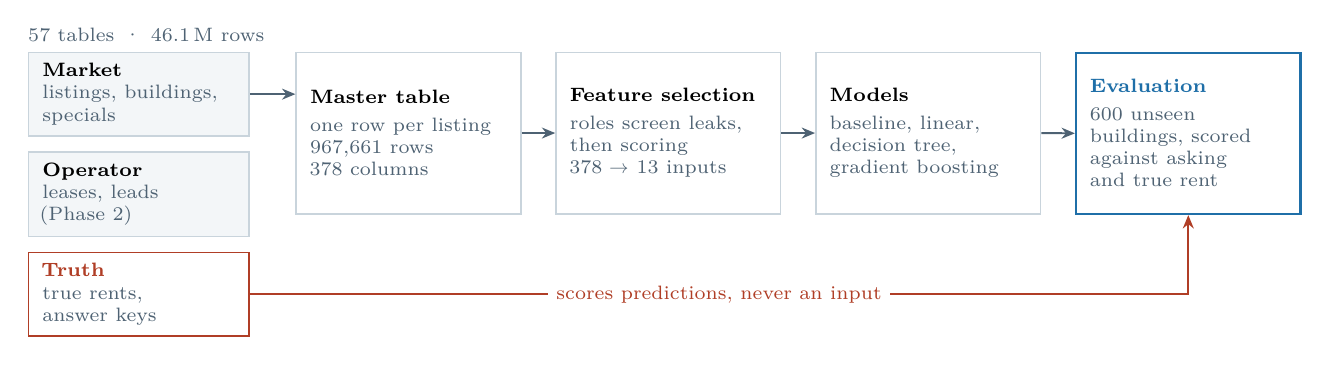
\begin{tikzpicture}[
  font=\scriptsize, >={Stealth[length=1.7mm, width=1.4mm]},
  box/.style={draw=rulecolor, line width=0.6pt, fill=white, align=flush left, anchor=north west,
              inner xsep=5pt, inner ysep=4pt},
  layer/.style={box, fill=wash, text width=2.45cm},
  stage/.style={box, text width=2.5cm, minimum height=2.05cm},
  flow/.style={->, draw=ink2, line width=0.7pt},
  h/.style={font=\scriptsize\bfseries\color{ink}},
]
\node[layer] (market) at (0, 0) {\textbf{Market}\\\textcolor{ink2}{listings, buildings,\\specials}};
\node[layer, below=1.8mm of market] (operator) {\textbf{Operator}\\\textcolor{ink2}{leases, leads\\(Phase 2)}};
\node[layer, below=1.8mm of operator, draw=brick, fill=white] (truth) {\textbf{\textcolor{brick}{Truth}}\\\textcolor{ink2}{true rents,\\answer keys}};
\node[anchor=south west, inner sep=0, text=ink2] at (0, 0.12) {\nSourceTables{} tables\enspace·\enspace\nSourceRowsM\,M rows};

\node[stage] (master) at (3.4, 0) {\textbf{Master table}\\[2pt]\textcolor{ink2}{one row per listing\\\nMasterRows{} rows\\\nMasterCols{} columns}};
\node[stage] (select) at (6.7, 0) {\textbf{Feature selection}\\[2pt]\textcolor{ink2}{roles screen leaks,\\then scoring\\\nMasterCols{} \(\to\) \nFeatures{} inputs}};
\node[stage] (models) at (10.0, 0) {\textbf{Models}\\[2pt]\textcolor{ink2}{baseline, linear,\\decision tree,\\gradient boosting}};
\node[stage, draw=accent, line width=0.8pt] (eval) at (13.3, 0) {\textbf{\textcolor{accent}{Evaluation}}\\[2pt]\textcolor{ink2}{\nTestBuildings{} unseen\\buildings, scored\\against asking\\and true rent}};

\draw[flow] (market.east) -- (master.west |- market.east);
\draw[flow] (master.east) -- (select.west);
\draw[flow] (select.east) -- (models.west);
\draw[flow] (models.east) -- (eval.west);
\draw[flow, draw=brick] (truth.east) -- (eval.south |- truth.east) -- (eval.south);
\node[fill=white, inner xsep=3pt, text=brick] at ($(truth.east)!0.5!(eval.south |- truth.east)$)
  {scores predictions, never an input};
\end{tikzpicture}

  \caption{From source tables to evaluation. The generator's truth layer feeds only the evaluation:
  it scores the predictions and is never a model input.}
  \label{fig:pipeline}
\end{figure}

\section{Methods}\label{sec:methods}

\revised{This section describes the synthetic and real data, how we prepared and explored them, how we
selected variables, and the models and concession extractor we built.}

\subsection{Data}\label{sec:data}

\revised{The original project proposal described a prepared seed dataset covering two to three U.S. metro
markets, roughly 10,000 to 20,000 buildings and 500,000 listing observations, with concession text,
property photos, and analyst-curated comparable sets. In our first meetings, we learned that the
real data was not yet available, so we began with synthetic data. As Accolade advised, we used the
synthetic data to develop and test the pipeline, not to select or tune models. The real Dwellsy
listing data arrived on October~22; we describe it at the end of this subsection.}

The synthetic data was built to conform to the structure of the real data: a market-relative
dataset, which mirrors the Dwellsy listings feed, and a demand pricing dataset, which mirrors a
property's own management-system records. It simulates \nBuildings{} apartment buildings in three
markets, Chicago (\nChicago{}), Dallas--Fort Worth (\nDfw{}), and Washington, DC (\nDc{}), from
\historyStart{} to \asOf{}, across \nSourceTables{} tables and \nSourceRowsM{} million rows. We
organize these tables in three layers (\cref{fig:pipeline}):

\begin{description}[leftmargin=1.5em, labelindent=0pt, font=\normalfont\bfseries]
  \item[Market] what a listings feed observes: buildings, floor plans, every listing with its dated
  price changes, and the free-text specials advertised with them.
  \item[Operator] full property-management records for \nPms{} buildings, including leases, guest
  cards, and a reference system's daily price recommendations, which we will use in Phase~2.
  \item[Truth] the values the generator drew before anything was observed, such as each floor plan's
  true market rent by month, each listing's true lease, and each building's latent quality and
  pricing policy.
\end{description}

\revised{The truth layer makes the synthetic data especially useful.} A real listings feed only
records what landlords asked, whereas this data also records what each unit was worth, so we can
evaluate whether a method recovers the market rent rather than whether it simply reproduces the
listings.

By default, the generator describes an unremarkable, stabilized building with 12-month leases, fully
priced and with nothing missing, and it then enables named edge cases on top. Attributes are masked:
\yearBuiltMasked{} of buildings are missing a year built and \storiesMasked{} a story count.
\nLeaseUp{} buildings are delivered partway through the history and lease up from empty,
\rmShare{} of buildings reprice daily under revenue management while the rest adjust by hand,
\nVacancySpikes{} vacancy spikes disrupt individual buildings, and \nRentControlled{} buildings in DC
are rent-controlled. Concessions appear in \nConcessionEvents{} advertised specials written in
varied prose. Because each edge case is named, the generator can double as a test harness for the
data-quality problems we expect in the real data.

One caution applies throughout. Because the generator builds rent from building attributes, a
flexible model can score well partly by recovering the generator's own formula. Therefore, we treat
our synthetic results as evidence that a method works when the data behaves as assumed, not as a
forecast of its accuracy on real listings.

\revised{The real data is a trial extract from Dwellsy, the listing provider. It covers \dwListings{}
listings of \dwUnits{} rental units in the Chicago and Washington, DC metropolitan areas between
\dwStart{} and \dwEnd{}, with the same 47 variables in both markets. We analyze Chicago first:
545,312 listings of 152,233 units, so a unit appears 3.6 times on average. The target is
\texttt{rent\_amount}, the advertised monthly rent, which is never missing. The main predictors are
the unit's bedrooms, bathrooms, and square footage, the building's year built and property type, its
ZIP code and coordinates, and the listing date. Most are nearly complete, but year built is 32\%
missing and half bathrooms 83\% missing. Unlike the synthetic data, the real data has no truth
layer, so we can score models only against asking rent.}

\subsection{Preprocessing}\label{sec:preprocessing}

\revised{We first merged} the \nMasterTables{} source tables relevant to rent prediction into a
master table with one row per listing, \nMasterRows{} listings by \nMasterCols{} columns. Building
and floor-plan attributes join one-to-many, while a listing's price history and advertised specials
are aggregated to the listing. Every join is checked for duplicated rows, and every column keeps the
name of its source table (for example, \texttt{market\_building\_\_year\_built}), so its origin stays
clear after any selection. \revised{We then reviewed each variable's content and
standardized its data type as a string, float, integer, date, or boolean.}

A column's name, however, does not tell us whether it can be used. We therefore also tagged each
column with a role (feature, label, latent, or leaky) and \revised{selected} inputs by role under a single rule:
an input must be known on the day the unit is listed. \Cref{fig:leakage} shows why this rule has to
be enforced by role rather than by correlation. Nine columns are the listing's own later prices and
correlate with asking rent at \(|r| \geq \minLeakyLevelR\), so they are easy to catch. Four more are
the same prices per square foot, with \(|r| \approx \psfAloneR\), no higher than the best legitimate
variable, so a correlation screen would keep them. Yet multiplied by square footage, they reproduce
asking rent to within 1\% for \psfExactShare{} of \nPsfRows{} listings (\(r = \psfTimesSqftR\)). A
model given these columns would score almost perfectly and learn nothing~\autocite{kaufman2012leakage}.

\begin{figure}[htbp]
  \centering
  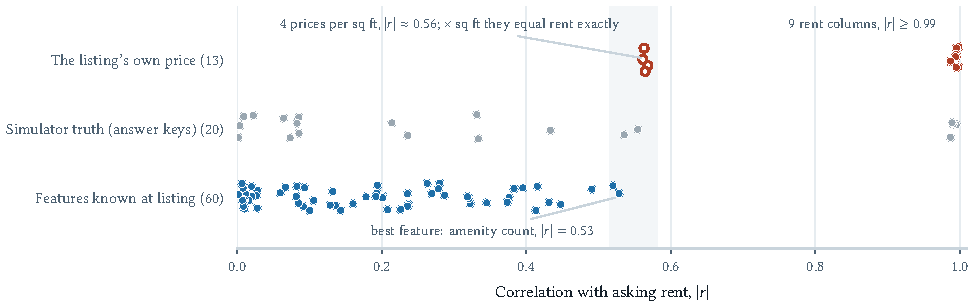
\includegraphics{leakage}
  \caption{Correlation of every numerical column with asking rent, by role. Variables known when a
  unit is listed (blue) reach \(|r| = \maxFeatureR\). The listing's own later prices (red) are
  leaks: nine rent columns are obvious, but four prices per square foot (open circles) fall in the
  shaded band beside the best variable, where correlation cannot tell them apart. Grey points are the
  generator's answer keys, never used as inputs.}
  \label{fig:leakage}
\end{figure}

\revised{For the real Chicago listings, our checks for invalid values found only one, a listing with a
non-positive square footage, so we kept every listing. We dropped half bathrooms and impute the
remaining missing values inside the modeling pipeline, fitted on the training set only: medians for
numerical variables and the most frequent value for categorical ones. Because units are listed
repeatedly, we split the data by rental unit into training (64\%), validation (16\%), and test
(20\%) sets. No unit appears in more than one set, so a model cannot score well by memorizing units
it has already seen.}

\subsection{Exploratory data analysis}\label{sec:eda}

Our exploratory analysis of the synthetic data focused on how rent varies across markets, unit types, and buildings, and on
which variables carry information about it. Median asking rent is \medRentDc{} in DC,
\medRentChicago{} in Chicago, and \medRentDfw{} in Dallas--Fort Worth (\cref{fig:map}). Between
\firstYear{} and \lastYear{} it rose by \growthChicago{} in Chicago and \growthDc{} in DC, while in
Dallas--Fort Worth it peaked in \dfwPeakYear{} and has since leveled off. Within each market, rent
generally rises with the number of bedrooms, but the spread within each bedroom count is wide
(\cref{fig:ladder} \revised{in \cref{app:figures}}), which suggests that location and building characteristics matter as much as the
size of the unit.

Unit size shows why the building level matters. Across all listings, square footage has a Pearson
correlation of \sqftOverallR{} with asking rent, but within a single building the correlation rises
to \sqftWithinR{}. In other words, size explains rent much better once the building is held fixed,
because buildings also differ in many other ways that affect price. \revised{Some promising variables,
however, are mostly missing:} \nSparseFees{} fee and parking variables have
Spearman correlations between \sparseRhoLo{} and \sparseRhoHi{} with rent, but are \sparseMissLo{} to
\sparseMissHi{} missing.

\revised{The real Chicago listings show the same building effect, though weaker: square footage
correlates with asking rent at 0.51 across all listings and 0.65 within a community, so comparable
selection should help on real data too. Two differences from the synthetic data matter for
modeling. Median asking rent in Chicago stayed between about \$1,500 and \$1,830 per quarter from
2021 to 2026, far flatter than the synthetic data's \growthChicago{} rise, so synthetic trends
should not guide real-data choices. The number of listings per quarter also fell from about 50,000
in 2021 to about 15,000 in 2025 and 2026, so most training data comes from the earliest years, and
we will also test on the most recent period.}

\begin{figure}[htbp]
  \centering
  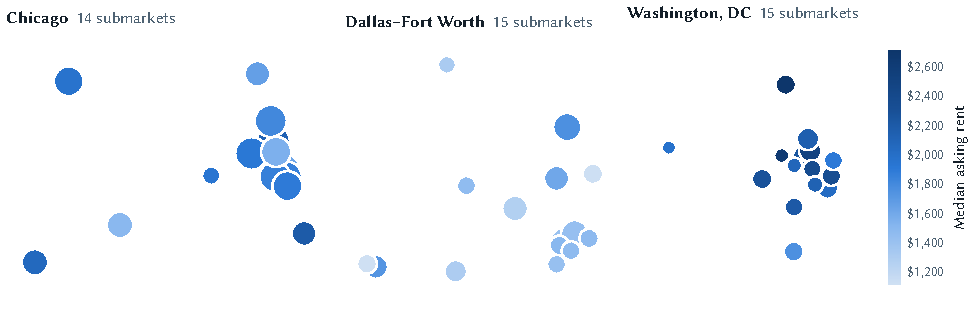
\includegraphics{rent_map}
  \caption{Median asking rent by submarket. Each circle is one submarket, sized by its number of
  listings and colored on one scale across the three markets.}
  \label{fig:map}
\end{figure}

\subsection{Feature selection}\label{sec:selection}

To narrow the \nMasterCols{} columns down to the model's inputs, we followed a staged funnel
(\cref{fig:funnel}, in \cref{app:figures}). After removing keys, answer keys, and leaky columns, \nFeatureCols{} columns
remain, of which \nKnownCols{} are known when a unit is listed. We then analyzed the numerical and
categorical variables separately.

For the numerical variables, we used two complementary approaches. The first scored every numerical
variable with Gini, gradient boosting importance, and Lasso, and kept \nKeptNumeric{} of the
\nNumCandidates{} candidates. The second applied univariate, bivariate, and multivariate stages in
sequence, narrowing 65 numerical predictors to 44 and then 18. The two selections agree on ten core
variables, led by unit size (Spearman correlation of \sqftSpearman{} with rent) together with
location, the building's amenity count and review score, its leasing exposure when the unit was
listed, and three measures of how often the building changes its prices.

\revised{For the categorical variables, we first profiled the 215 boolean and 28 categorical predictors
against the target. We found that cardinality has to be judged per building rather than per row.} A street address is only 0.31\% distinct across listings but 99.97\% distinct across
buildings, so it is effectively a building identifier rather than a category. We therefore excluded
identifiers and chose which categorical variables to keep based on their importance on buildings the
model had not seen. Six of the \nCatCandidates{} candidates are kept: property class, ZIP code, floor
plan name, unit name, the predicted story bucket, and management company. On their own, they reach
an \(R^2\) of 0.55 on held-out buildings.


\subsection{Models}\label{sec:models}

Our initial models, developed using synthetic data, predict the first asking rent of a listing, 
the price posted when the unit comes on the market. As inputs we use \nFeatures{} numerical 
variables known at that point: unit size, bedrooms,
bathrooms, and floor; the building's amenities, review score, size, age, and application fee; its
location; and the number of units sharing the floor plan. We compared three models: linear
regression as an interpretable reference, a decision tree for its readable splits, and gradient
boosting~\autocite{friedman2001greedy} to capture nonlinear relationships. Missing values are imputed
with the median for linear regression and the decision tree, while gradient boosting, implemented as
scikit-learn's histogram-based gradient boosting~\autocite{ke2017lightgbm, pedregosa2011scikit},
handles them natively. As a reference point, we also include a naive baseline that predicts the
median rent for the listing's market and bedroom count. \Cref{app:models} lists the settings.

\revised{On the real Chicago listings, we compared five regression models: linear regression, a decision
tree, a random forest, histogram-based gradient boosting, and a baseline that predicts the mean
training rent. They use eight predictors: bedrooms, full bathrooms, square footage, year built, ZIP
code, property type, and the listing's year and month, with ZIP code and property type one-hot
encoded. We compare the models on the validation set and keep the test set for the final model. To
test whether exact location adds information beyond ZIP code, we also fit a Ridge regression with
spline transformations of latitude and longitude.}

\subsection{Concession extraction}\label{sec:concession-methods}

As a first step toward Phase~2, we built a rule-based extractor for concession terms. Advertised
specials are free text, such as ``Enjoy the first month free on a 13-month lease,'' and Phase~2 needs
their value in dollars to compute effective rent. We found that the concession type is already
recorded in the market data and agrees with the truth layer for every one of the
\nConcessionEvents{} specials, so only the value has to be extracted from the text. The extractor
reads the amount, its basis (months free or dollars), and the lease term, and we score it against
the truth layer.

\section{Preliminary results}\label{sec:results}

\revised{This section reports our results.
\Cref{sec:evaluation,sec:market-rent,sec:errors,sec:drivers,sec:concessions,sec:pipeline} cover the
synthetic data, where the truth layer lets us score predictions against the true market rent.
\Cref{sec:real-results} gives our first results on the real Chicago listings.}

\subsection{Evaluation}\label{sec:evaluation}

We evaluate every model on buildings it has never seen. Listings are split by building,
\nTrainBuildings{} for training and \nTestBuildings{} for testing, so no building contributes to
both. With about \listingsPerBuilding{} listings per building, a split by listing would let a model
memorize buildings and overstate its accuracy. Our primary metric is the median absolute percentage
error,
\[
  \mathrm{MdAPE} \;=\; \operatorname*{median}_{i}\, \frac{\lvert \hat{y}_i - y_i \rvert}{y_i},
\]
which reads directly as a typical miss, compares fairly across markets with different rent levels,
and is not dominated by the few luxury units with the largest dollar errors. We also report the mean
absolute error (MAE) in dollars and \(R^2\). \revised{We also score} each model twice: against the
asking rent it was trained to predict, and against the generator's true market rent for the same
floor plan and month, a comparison that only synthetic data allows. \revised{On the real Chicago
data, models are evaluated on held-out rental units. That data has no truth layer, so we compare
models by MAE, \(R^2\), and the root mean squared error (RMSE), which penalizes large misses more
heavily. We will add MdAPE so that the two datasets can be compared directly.}

\subsection{Market rent}\label{sec:market-rent}

\Cref{tab:models} compares the three models with the naive baseline. Gradient boosting performs
best, cutting the baseline's median error by \errorReduction{}, from \baseMdape{} to \gbmMdape{}, with
an MAE of \gbmMae{} and an \(R^2\) of \gbmRsq{} on the \nTestListings{} listings of the held-out
buildings. It also lowers MAE by \gbmVsLinear{} compared with linear regression. Because the data
are synthetic and a single test set was used to compare the models, these results are a working
baseline rather than a model selection.

The last row of \cref{tab:models} is the most informative. A listing's own asking rent sits within
\noiseFloor{} of the true market rent, which means asking rent is a reliable training target, and
each model's error against the true rent (\gbmMdapeTrue{} for gradient boosting) matches its error
against the asking rent. The remaining error therefore does not come from noise in the listings. It
comes from information about each building that our \nFeatures{} variables do not capture.
\revised{Nearby comparable buildings carry that information, which is why comparable-property selection
is our next step.}

\begin{table}[htbp]
  \caption{Performance on \nTestBuildings{} held-out buildings (\nTestListings{} listings). MdAPE is
  measured against each listing's asking rent and against the generator's true market rent for its
  floor plan and month. The last row is how far the listing itself sits from the truth.}
  \label{tab:models}
  \centering\small
  \begin{tabular}{@{}l S[table-format=3.0] S[table-format=1.2] S[table-format=2.1] S[table-format=2.1]@{}}
\toprule
 & {MAE} & {\(R^2\)} & \multicolumn{2}{c}{MdAPE (\%)} \\
\cmidrule(l){4-5}
Model & {(\$)} & & {vs.\ asking} & {vs.\ true} \\
\midrule
Naive baseline (market \(\times\) bedrooms median) & 443 & 0.30 & 21.0 & 21.0 \\
Linear regression & 285 & 0.70 & 13.0 & 13.1 \\
Decision tree & 302 & 0.65 & 13.3 & 13.2 \\
\textbf{Gradient boosting} & 235 & 0.79 & 10.6 & 10.6 \\
\midrule
The listing's own asking rent & {---} & {---} & {---} & 2.8 \\
\bottomrule
\end{tabular}

\end{table}

\begin{figure}[htbp]
  \centering
  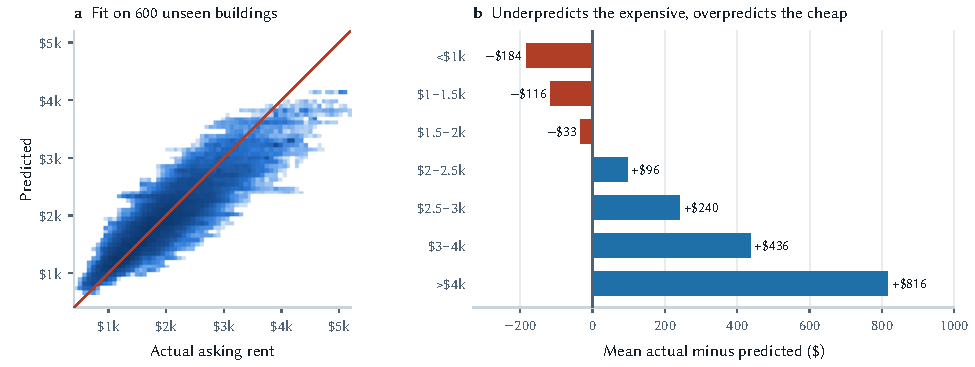
\includegraphics{fit}
  \caption{Predictions on held-out buildings. (a)~Each square is a bin of listings, darker where more
  fall; the red line is perfect prediction. (b)~Mean error by actual rent: the model pulls toward the
  middle, overpredicting the cheapest units by \biasLow{} and underpredicting the most expensive by
  \biasHigh{}.}
  \label{fig:fit}
\end{figure}

\subsection{Where the model errs}\label{sec:errors}

Errors grow with rent (\cref{fig:fit}). The model pulls its predictions toward the middle: low rents
are overpredicted and high rents underpredicted, by an average of \biasLow{} for units under \$1,000
and \biasHigh{} for units above \$4,000. \Cref{fig:segments} breaks the error down by segment. It is
largest for class C buildings and for units with four or more bedrooms, and the bias differs by
property class: class A buildings are underpredicted and class C buildings overpredicted. This
pattern is consistent with the model not yet using property class, the strongest categorical
variable we identified. Lease-up buildings, which we expected to be harder, are in fact predicted
slightly better than stabilized ones (\mdapeLeaseUp{} against \mdapeStabilized{}).

\begin{figure}[htbp]
  \centering
  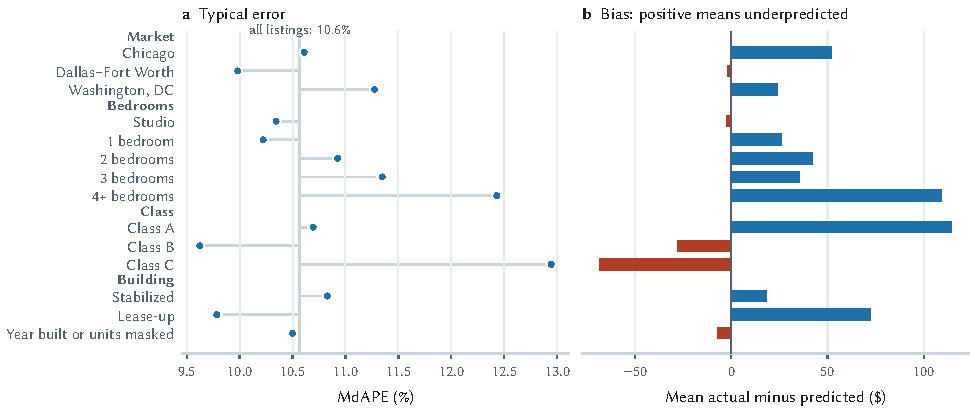
\includegraphics{segments}
  \caption{Error by segment on held-out buildings. (a)~MdAPE; the vertical line is the overall
  \gbmMdape{}. (b)~Mean actual minus predicted rent. Class A is underpredicted and class C
  overpredicted, consistent with the model lacking property class, the strongest categorical
  candidate in \cref{fig:drivers}.}
  \label{fig:segments}
\end{figure}

\subsection{What drives the predictions}\label{sec:drivers}

\Cref{fig:drivers}a shows how much each input contributes on unseen buildings, measured by the
increase in MAE when that input is shuffled. Unit size matters most, adding \topFeatureDmae{} to the
MAE when shuffled, followed by latitude, the building's amenity count, and longitude. Location ranks
high in this test, consistent with our exploratory analysis, while bathrooms and the number of units
sharing the floor plan add almost nothing once the other inputs are known. \Cref{fig:drivers}b and~c
show why we select categorical variables on held-out importance rather than in-sample fit: state and
metro area fit the training buildings well but add nothing on unseen ones, while property class is
by far the most useful.

\begin{figure}[htbp]
  \centering
  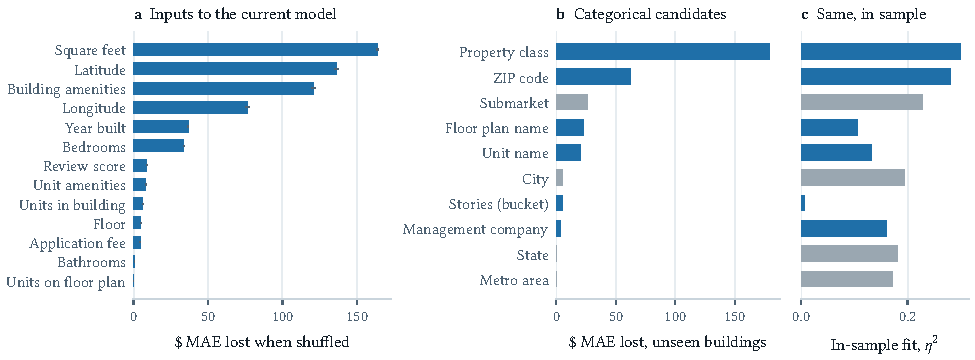
\includegraphics{drivers}
  \caption{Which inputs matter on unseen buildings. (a)~Dollars of mean absolute error added when
  each of the model's \nFeatures{} inputs is shuffled. (b)~The same measure for the categorical
  candidates, blue where kept. (c)~Their in-sample fit: state and metro area fit the training
  buildings but add nothing on unseen ones.}
  \label{fig:drivers}
\end{figure}

\subsection{Concession extraction}\label{sec:concessions}

The extractor gets the amount right for \concAmountAcc{} of the \concN{} specials that state their
terms, and values the concession within 5\% for \concWithinFive{} of them (\cref{fig:concessions}, in
\cref{app:figures}).
Accuracy depends on how the text was written. On specials written by a language model the rules are
right \concLlm{} of the time, but on the generator's template text they are right only \concGrammar{}
of the time, because these specials often quote a dollar amount or a net effective rent where the
truth layer records months free. Every dollar-denominated special is read correctly, while specials
offering free months reach \concMonthsFree{}.


\subsection{Pipeline and reproducibility}\label{sec:pipeline}

All of our code and outputs are shared through the team's GitHub repository. Three commands rebuild
the master table from the public download, and 59 join checks verify that the merged table is
complete and consistent. \revised{The same code recomputes every
synthetic-data number, table, and figure in this report from the data, so the report stays
consistent with the models behind it.}


\subsection{Preliminary results on real Dwellsy data}\label{sec:real-results}

\revised{\Cref{tab:real-models} compares the five models on the Chicago validation set.}

\begin{table}[htbp]
  \caption{\revised{Preliminary performance on real Chicago listings, measured on the validation set
  (rental units held out from training).}}
  \label{tab:real-models}
  \centering\small
  \revised{\begin{tabular}{@{}lrrr@{}}
    \toprule
    Model & MAE (\$) & RMSE (\$) & \(R^2\) \\
    \midrule
    \textbf{Gradient boosting} & 229 & 396 & 0.83 \\
    Random forest & 291 & 465 & 0.77 \\
    Linear regression & 335 & 552 & 0.68 \\
    Decision tree & 346 & 533 & 0.70 \\
    Baseline (mean training rent) & 669 & 970 & 0.00 \\
    \bottomrule
  \end{tabular}}
\end{table}

\revised{Gradient boosting performs best, with an MAE of \$229 and an \(R^2\) of 0.83, against \$669 and
0.00 for the baseline. As on the synthetic data, it beats linear regression and a single decision
tree, and the random forest comes second. The two tree ensembles outperform the simpler models,
which suggests that rent depends on interactions between unit characteristics and location. We will
tune these models and test others before choosing one.}

\revised{The Ridge regression tests whether exact location adds information beyond ZIP code. Adding spline
transformations of latitude and longitude lowered validation MAE by only \$1.78 and raised \(R^2\) by
0.0024, so in this model ZIP code already captures most of the location signal.}

% Section 4. Suggested owner: Viviana.  Budget: ~1 page.
\section{Discussion}\label{sec:discussion}

\subsection{Conclusion}
\brief{Viviana}{~0.4 page}{%
Three or four takeaways, each tied to a result in \cref{sec:results}: a defensible pipeline with
leakage guarded by role; boosting halves the baseline's error on unseen buildings; the remaining
error is missing information, not label noise; concession type is free and concession value is
where the work is.}

\subsection{Future work through April}
\brief{Viviana}{~0.6 page}{%
Each step justified by an observation. Comp selection and a similarity-weighted comp baseline,
because the error is missing building information (\cref{sec:market-rent}). Ranges with tested
coverage, through quantile models or conformal prediction \autocite{angelopoulos2023gentle}.
Plain-language reasons from SHAP values \autocite{lundberg2017unified}. A time-based test on the
latest months. Phase 2: the demand-conversion recommender. Moving the pipeline to the real Dwellsy
extract, which shares the listing-and-unit structure but lacks the concession fields its
documentation lists.}

\section*{Contributions}
\addcontentsline{toc}{section}{Contributions}
\todo{Each member: confirm or edit your paragraph.}

\textbf{Maria Gonzalez Llama.} Maria coordinated the team's weekly tasks and early communication with
our mentor, prepared the preliminary note on project scope, and reviewed a German study on
comparable-property valuation for the literature review. She developed the slides for our first
capstone presentation, built the first model-training notebook with a leakage review and a grouped
split, compared linear regression, a decision tree, and gradient boosting, and analyzed the errors by
rent level. She has also begun preparing the real Dwellsy data for modeling.

\textbf{Viviana Hanampa Castillo.} Viviana coordinated our first meeting with Accolade and the team's
schedule, and reviewed a study of spatial market segments in the Spanish markets. She wrote the Gini
analysis and the report of string and numerical variables, scored all 108 numerical variables with
Gini, gradient boosting, and Lasso, and built the correlation report, the decision table, and the
exploratory notebook for numerical variables. She also reorganized the repository by project phase,
with notebook filters and join checks.

\textbf{Shikha Mehta.} Shikha reviewed competitor sites and multifamily rental websites to identify
the variables we would need, and papers on multimodal models, Zillow's home value index methodology,
and model evaluation for rent prediction. She analyzed the numerical variables with Pearson and
Spearman correlations, mutual information, within-building correlation, and permutation importance,
wrote the plotting script for our exploratory figures, and found that size explains rent much better
within a building than across all listings. She also wrote several of our weekly reports.

\textbf{Matthew Reynolds.} Matthew researched listing data sources and established methods for rent
prediction, set up the team's GitHub repository, and reviewed work on algorithmic pricing and TWFE
models. He was the first to work with the data, merging \nMasterTables{} tables into the
\nMasterCols{}-column master table, and built the categorical selection based on held-out importance
and the Phase~2 concession extractor. He handled communication with our sponsor, and built this
report's figures and the pipeline that generates it.

\textbf{Lady Infante Acosta.} Lady reviewed a São Paulo study on rental pricing to identify
geospatial features, and standardized the data types of every variable in a script that is part of
our processing pipeline. She built the staged selection funnel with univariate, bivariate, and
multivariate stages, narrowing 65 numerical predictors to 18, and profiled the 215 boolean and 28
categorical predictors against the target. She has also begun the categorical analysis of the real
Dwellsy data.


\printbibliography[heading=bibintoc, title={References}]

\appendix
% Appendices: outside the 8-10 page limit.
\section{Data dictionary}\label{app:dictionary}
\brief{Matthew}{as needed}{%
The master table's column groups with counts by role, from \texttt{data/master\_columns.csv}.}

\section{Model specifications}\label{app:models}
\brief{Maria}{as needed}{%
Hyperparameters for each model in \cref{tab:models}, and the feature list.}


\end{document}
